% ============================================================================
%  ECE 431 -- Sheet 7 Solutions
%  Style: sheet-answering-style.md
% ============================================================================

\begin{question}[Question 1]
Find the energy gap and refractive index of Ga$_{0.7}$Al$_{0.3}$As, and the composition of the alloy Ga$_{1-x}$Al$_x$As that emits at 800nm. If these compositions are used to make a double hetero-structure P-n-N diode, find the lattice mismatch ($\Delta a/a$) at the hetero-junctions, and the relative refractive index difference of the resulting slab waveguide. Is this slab single-mode for a thickness d = 0.2 \si{\micro\meter}? Use graphs or tables and assume linear dependence of the material parameters on the composition fraction x.
\end{question}

\textbf{\large Solution --- Question 1}

\textbf{Step 1: Double Heterostructure (DH) Principles \& Cladding Properties}

To design a Double Heterostructure (DH) laser, the active layer (where light is generated) is sandwiched between two cladding layers. For proper operation, the active layer must have:
\begin{itemize}
    \item A \textbf{smaller bandgap} than the cladding layers to trap electrons and holes (carrier confinement).
    \item A \textbf{higher refractive index} than the cladding layers to act as a dielectric waveguide and confine the generated photons (optical confinement).
\end{itemize}

We are given the cladding layer composition: $\text{Ga}_{0.7}\text{Al}_{0.3}\text{As}$, meaning the Aluminum mole fraction is $x = 0.3$. 
To find the physical properties of this ternary alloy, we use \textbf{Vegard's law}, which assumes that the properties of an alloy vary linearly between the properties of its constituent binary compounds (GaAs and AlAs). 

Given the standard bandgaps $E_{g,\text{GaAs}} = 1.424\,\text{eV}$ and $E_{g,\text{AlAs}} = 2.16\,\text{eV}$, the bandgap of the cladding layer is calculated by linear interpolation:
\begin{align*}
  E_{g,\text{clad}} &= 0.7 E_{g,\text{GaAs}} + 0.3 E_{g,\text{AlAs}} = 0.7(1.424) + 0.3(2.16) = 1.645\,\text{eV}
\end{align*}

Similarly, using the common linear approximation for the refractive index of $\text{Al}_x\text{Ga}_{1-x}\text{As}$ ($n \approx 3.5 - 0.62x$), the cladding refractive index is:
\begin{equation*}
  n_{\text{clad}} = 3.5 - 0.62(0.3) = 3.314
\end{equation*}

\textbf{Step 2: Composition and properties for the Active Layer}

The laser is designed to emit light at a wavelength of $\lambda = 800\,\text{nm}$. The energy of the emitted photons corresponds exactly to the bandgap of the active layer. We calculate the required bandgap using $E_g = \frac{hc}{\lambda}$:
\begin{equation*}
  E_{g,\text{active}} = \frac{1.24\,\text{eV}\cdot\mu\text{m}}{0.8\,\mu\text{m}} = 1.55\,\text{eV}
\end{equation*}

Now, we use linear interpolation again to find the Aluminum fraction $x_{\text{active}}$ that gives this exact bandgap:
\begin{equation*}
  E_{g,\text{active}} = (1-x)E_{g,\text{GaAs}} + x E_{g,\text{AlAs}} \implies 1.55 = (1-x)(1.424) + x(2.16)
\end{equation*}
Solving for $x$:
\begin{equation*}
  x_{\text{active}} = \frac{1.55 - 1.424}{2.16 - 1.424} \approx 0.171 \approx 0.17
\end{equation*}
So the active layer is $\text{Ga}_{0.83}\text{Al}_{0.17}\text{As}$. Using this composition, its refractive index is:
\begin{equation*}
  n_{\text{active}} = 3.5 - 0.62(0.17) = 3.395
\end{equation*}

\textit{Conceptual check:} Notice that $E_{g,\text{active}} (1.55\,\text{eV}) < E_{g,\text{clad}} (1.645\,\text{eV})$ and $n_{\text{active}} (3.395) > n_{\text{clad}} (3.314)$. Both confinement conditions for a DH laser are perfectly met.

\textbf{Step 3: Lattice mismatch at the heterojunction}

A critical requirement for heterojunctions is that the crystal lattices of the two materials must match closely. A large lattice mismatch creates defects and dislocations at the interface, which act as non-radiative recombination centers and destroy the laser's efficiency.

We calculate the lattice constants using Vegard's law and the known constants ($a_{\text{GaAs}} = 5.6533\,\text{\AA}$ and $a_{\text{AlAs}} = 5.6605\,\text{\AA}$):
\begin{align*}
  a_{\text{clad}} (x=0.3) &= 0.3(5.6605) + 0.7(5.6533) = 5.65546\,\text{\AA} \\
  a_{\text{active}} (x=0.17) &= 0.17(5.6605) + 0.83(5.6533) = 5.65452\,\text{\AA}
\end{align*}
The fractional lattice mismatch $\frac{\Delta a}{a}$ is defined relative to the active layer:
\begin{equation*}
  \frac{\Delta a}{a} = \frac{|a_{\text{clad}} - a_{\text{active}}|}{a_{\text{active}}} = \frac{|5.65546 - 5.65452|}{5.65452} \approx 1.66 \times 10^{-4} \approx 0.017\%
\end{equation*}
This mismatch is extremely small ($<0.1\%$), which is why the $\text{AlGaAs/GaAs}$ material system is so successful for making high-quality lasers.

The relative step change in the refractive index (often denoted as $\Delta$) is:
\begin{equation*}
  \frac{\Delta n}{n_{\text{active}}} = \frac{n_{\text{active}} - n_{\text{clad}}}{n_{\text{active}}} = \frac{3.395 - 3.314}{3.395} \approx 0.024 \quad (2.4\%)
\end{equation*}

\textbf{Step 4: Waveguide single-mode condition}

The active layer acts as a symmetric dielectric slab waveguide. To ensure that the laser beam maintains a clean, single transverse profile, the waveguide must be designed to support only the fundamental mode. 
This is governed by the normalized frequency (or $V$-parameter). For a symmetric slab, the condition for single-mode operation is $V < \pi$.

Using the active layer thickness $d = 0.2\,\mu\text{m}$, we calculate $V$:
\begin{equation*}
  V = \frac{2\pi}{\lambda} d \sqrt{n_{\text{active}}^2 - n_{\text{clad}}^2} = \frac{2\pi}{0.8\,\mu\text{m}} (0.2\,\mu\text{m}) \sqrt{3.395^2 - 3.314^2} \approx 1.16
\end{equation*}
Since $V \approx 1.16$, which is strictly less than $\pi \approx 3.14$, the waveguide operates deep in the single-mode regime. Only the fundamental transverse mode is supported.


\begin{question}[Question 2]
A double-heterostructure semiconductor laser is made of an active layer of Al$_x$Ga$_{1-x}$As surrounded by upper and lower cladding layers of Al$_{0.6}$Ga$_{0.4}$As, as shown in the figure.\\
\begin{center}
  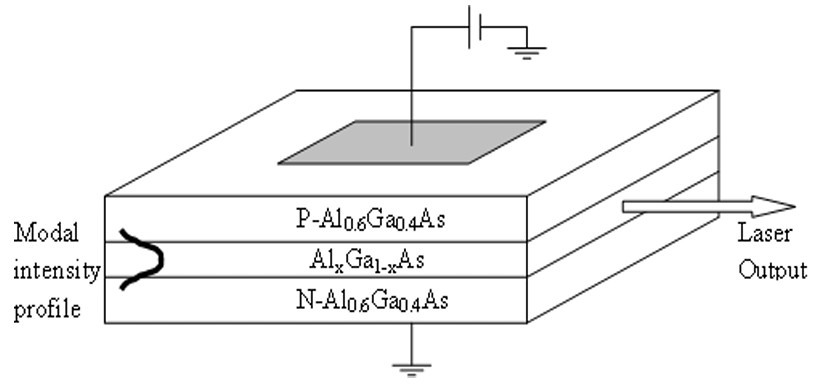
\includegraphics[width=0.6\textwidth]{../Figures/Sheet 7/q2_a.jpg}
\end{center}
(a) Use the data in the table below to find\\
(1) The Aluminum mole fraction, $x$, in the active layer to emit photons of energy 1.6 eV.\\
(2) The energy gap discontinuity, $\Delta E_g$, the conduction band edge discontinuity, $\Delta E_c$, and the valence band edge discontinuity, $\Delta E_v$, at the hetrojunctions.

\begin{center}
\begin{tabular}{|l|c|c|}
\hline
 & $0 \le x \le 0.45$ & $0.45 \le x \le 1.0$ \\
\hline
Energy Gap (eV) & $1.424 + 1.247x$ & $1.424 + 1.247x + 1.147(x - 0.45)^2$ \\
\hline
Electron Affinity (eV) & $4.07 - 1.1x$ & $3.64 - 0.14x$ \\
\hline
\end{tabular}
\end{center}


\noindent\begin{minipage}[c]{0.51\linewidth}
(b) The figure shown plots the refractive index of Al$_x$Ga$_{1-x}$As against photon energy (with $x$ increments of 0.1). Use this figure to find the refractive index in the active layer and in the cladding layers.\\[1ex]
(c) Find the maximum thickness of the active layer to support a single transverse mode.\\
(d) Mention two advantages of a double-heterostructure laser compared to a single-heterojunction laser?
\end{minipage}\hfill
\begin{minipage}[c]{0.45\linewidth}
  \centering
  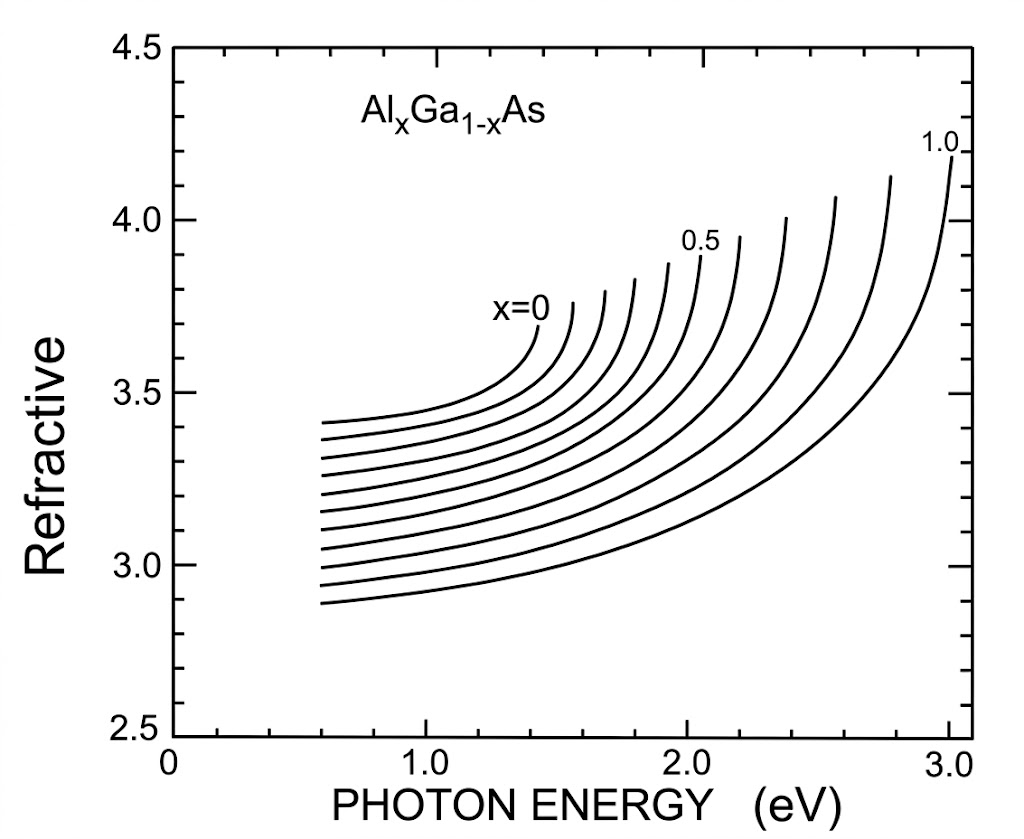
\includegraphics[width=\linewidth]{../Figures/Sheet 7/q2_b.jpg}
\end{minipage}
\end{question}

\textbf{\large Solution --- Question 2}

\textbf{(a) Active layer composition and energy band discontinuities}

\textbf{(1) Active layer composition ($x$):}
For the active layer to emit photons of exactly $1.6\,\text{eV}$, its bandgap must match this photon energy ($E_g = 1.6\,\text{eV}$). To ensure efficient light emission, the active layer must be a direct bandgap semiconductor, which corresponds to the $0 \le x \le 0.45$ regime in the provided table.
Setting the direct bandgap equation to $1.6\,\text{eV}$:
\begin{equation*}
  E_g = 1.424 + 1.247x = 1.6 \implies 1.247x = 0.176 \implies x \approx 0.141
\end{equation*}
So the active layer is $\text{Al}_{0.141}\text{Ga}_{0.859}\text{As}$.

\textbf{(2) Band edge discontinuities ($\Delta E_g$, $\Delta E_c$, $\Delta E_v$):}
First, we calculate the bandgap of the surrounding cladding layers ($x = 0.6$). Since $x > 0.45$, the cladding is an indirect bandgap material. We use the second equation from the table:
\begin{equation*}
  E_{g,\text{clad}} = 1.424 + 1.247(0.6) + 1.147(0.6 - 0.45)^2 \approx 2.198\,\text{eV}
\end{equation*}
The total energy gap discontinuity between the cladding and the active layer is:
\begin{equation*}
  \Delta E_g = E_{g,\text{clad}} - E_{g,\text{active}} = 2.198 - 1.6 = 0.598\,\text{eV}
\end{equation*}

To find how this total discontinuity $\Delta E_g$ is split between the conduction band ($\Delta E_c$) and the valence band ($\Delta E_v$), we use the \textbf{electron affinity ($\chi$)}. Electron affinity is the energy required to excite an electron from the bottom of the conduction band ($E_c$) to the vacuum level. Therefore, the step in the conduction band ($\Delta E_c$) is simply the difference in electron affinities between the two materials.

Using the affinity equations from the table:
\begin{align*}
  \chi_{\text{active}} \,(x = 0.141) &= 4.07 - 1.1(0.141) = 3.915\,\text{eV} \\
  \chi_{\text{clad}} \,(x = 0.6) &= 3.64 - 0.14(0.6) = 3.556\,\text{eV}
\end{align*}
The conduction band discontinuity acts as the potential barrier confining the electrons:
\begin{equation*}
  \Delta E_c = |\chi_{\text{active}} - \chi_{\text{clad}}| = 3.915 - 3.556 = 0.359\,\text{eV}
\end{equation*}
The remainder of the bandgap discontinuity forms the valence band barrier, which confines the holes:
\begin{equation*}
  \Delta E_v = \Delta E_g - \Delta E_c = 0.598 - 0.359 = 0.239\,\text{eV}
\end{equation*}

\textbf{(b) Refractive indices from the plot}

The refractive index is a property experienced by the specific electromagnetic wave traveling through the material. Since the laser emits photons at $1.6\,\text{eV}$, the light propagating through \textit{both} the core and the cladding has exactly this energy. Therefore, we must evaluate both refractive indices at $h\nu = 1.6\,\text{eV}$ on the horizontal axis, \textit{not} at their respective bandgap energies!

\begin{itemize}
    \item \textbf{For the active core ($x \approx 0.14$):} We look at $h\nu = 1.6\,\text{eV}$ and estimate slightly below the $x=0.1$ curve, yielding $n_{\text{core}} \approx 3.75$.
    \item \textbf{For the cladding ($x = 0.6$):} We stay at $h\nu = 1.6\,\text{eV}$ and follow the $x=0.6$ curve, yielding $n_{\text{cladding}} \approx 3.28$. (Notice that the light energy $1.6\,\text{eV}$ is well below the cladding bandgap of $\sim 2.2\,\text{eV}$, ensuring the cladding is perfectly transparent to the laser light).
\end{itemize}

\textbf{(c) Maximum single-mode thickness ($d_{\text{max}}$)}

For a symmetric dielectric slab waveguide, the cutoff for the first higher-order transverse mode occurs when the normalized frequency parameter $V$ reaches $\pi$. To guarantee that only the fundamental single mode propagates, the thickness $d$ must satisfy $V \le \pi$.

The emission wavelength is $\lambda_L = \frac{hc}{E_g} = \frac{1.24\,\text{eV}\cdot\mu\text{m}}{1.6\,\text{eV}} = 0.775\,\mu\text{m}$.
Setting $V = \pi$:
\begin{equation*}
  V = \frac{2\pi}{\lambda_L} d_{\text{max}} \sqrt{n_{\text{core}}^2 - n_{\text{cladding}}^2} = \pi \implies d_{\text{max}} = \frac{\lambda_L}{2\sqrt{n_{\text{core}}^2 - n_{\text{cladding}}^2}}
\end{equation*}
Substituting our values:
\begin{equation*}
  d_{\text{max}} = \frac{0.775}{2\sqrt{3.75^2 - 3.28^2}} \approx \frac{0.775}{2(1.817)} \approx 0.213\,\mu\text{m}
\end{equation*}
The active layer must not exceed $0.213\,\mu\text{m}$ to remain strictly single-mode.

\textbf{(d) Advantages of double-heterostructure (DH) lasers}

Compared to a simple homojunction or single-heterojunction laser, a DH laser offers two massive physical advantages that dramatically lower the threshold current density ($J_{\text{th}}$):
\begin{enumerate}
  \item \textbf{Dual Carrier Confinement:} The energy band discontinuities ($\Delta E_c$ and $\Delta E_v$) act as potential walls on \textit{both} sides of the active region. This forces electrons and holes to remain tightly confined in the narrow active layer, preventing them from diffusing away before they can radiatively recombine.
  \item \textbf{Optical Waveguiding:} Because the active layer has a higher refractive index than both cladding layers ($n_{\text{core}} > n_{\text{cladding}}$), it forms a natural dielectric waveguide. This traps the generated photons within the same physical space as the confined carriers, maximizing stimulated emission efficiency.
\end{enumerate}


\begin{question}[Question 3]
Derive an expression for the injection efficiency across a p-n homo-junction formed in a direct band-gap semiconductor in which radiative recombination dominates other recombination processes. Hence calculate the injection efficiency in a p$^+$n GaAs diode in which N$_A = 10^{24}$ m$^{-3}$ and N$_D = 10^{21}$ m$^{-3}$. Put the recombination coefficient r = $10^{-16}$ m$^3$/s and the diffusion constant, D$_e = 21$ D$_h$.
\end{question}

\textbf{\large Solution --- Question 3}

\textbf{Derivation of injection efficiency.}

In a p-n homojunction, the minority carrier injection currents across the depletion region are given by diffusion currents at the boundaries:
\begin{equation*}
  J_e = -e D_e \frac{\partial \Delta N}{\partial x} \Big|_{x=0} = e \frac{D_e \Delta N(0)}{L_e}
\end{equation*}
\begin{equation*}
  J_h = -e D_h \frac{\partial \Delta P}{\partial y} \Big|_{y=0} = e \frac{D_h \Delta P(0)}{L_h}
\end{equation*}
where the excess carrier concentrations at the edges are:
\begin{equation*}
  \Delta N(0) = n_{p0}\left(e^{e V_A / k_B T} - 1\right) \quad \text{and} \quad \Delta P(0) = p_{n0}\left(e^{e V_A / k_B T} - 1\right)
\end{equation*}
Substituting these into the current expressions:
\begin{equation*}
  J_e = e \frac{D_e n_{p0}}{L_e}\left(e^{e V_A / k_B T} - 1\right) \quad \text{and} \quad J_h = e \frac{D_h p_{n0}}{L_h}\left(e^{e V_A / k_B T} - 1\right)
\end{equation*}

The current injection efficiency for electrons is:
\begin{equation*}
  \eta_j = \frac{J_e}{J_e + J_h} = \frac{1}{1 + \frac{J_h}{J_e}} = \frac{1}{1 + \frac{D_h L_e p_{n0}}{D_e L_h n_{p0}}}
\end{equation*}
Using the equilibrium minority carrier relation ($p_{n0} = n_i^2/N_D$ and $n_{p0} = n_i^2/N_A$), we have $\frac{p_{n0}}{n_{p0}} = \frac{N_A}{N_D}$:
\begin{equation*}
  \eta_j = \frac{1}{1 + \frac{D_h L_e N_A}{D_e L_h N_D}}
\end{equation*}

Given that radiative recombination dominates, the lifetime of electrons in the p-side and holes in the n-side are:
\begin{equation*}
  \tau_e = \frac{1}{r N_A} \quad \text{and} \quad \tau_h = \frac{1}{r N_D}
\end{equation*}
The corresponding diffusion lengths are:
\begin{equation*}
  L_e = \sqrt{D_e \tau_e} = \sqrt{\frac{D_e}{r N_A}} \quad \text{and} \quad L_h = \sqrt{D_h \tau_h} = \sqrt{\frac{D_h}{r N_D}}
\end{equation*}
Taking the ratio of the diffusion lengths:
\begin{equation*}
  \frac{L_e}{L_h} = \sqrt{\frac{D_e N_D}{D_h N_A}}
\end{equation*}
Substituting this ratio back into the efficiency expression:
\begin{equation*}
  \eta_j = \frac{1}{1 + \frac{D_h}{D_e}\sqrt{\frac{D_e N_D}{D_h N_A}}\frac{N_A}{N_D}} = \boxed{\frac{1}{1 + \sqrt{\frac{D_h N_A}{D_e N_D}}}}
\end{equation*}

\textbf{Numerical calculation for $p^+n$ GaAs diode.}

Given $N_A = 10^{24}\,\text{m}^{-3}$, $N_D = 10^{21}\,\text{m}^{-3}$, and $D_e = 21 D_h$:
\begin{equation*}
  \frac{L_e}{L_h} = \sqrt{21 \times \frac{10^{21}}{10^{24}}} = \sqrt{\frac{21}{1000}} \approx 0.1449
\end{equation*}
Substituting into our derived efficiency formula:
\begin{equation*}
  \eta_j = \frac{1}{1 + \frac{1}{21}\sqrt{21 \times \frac{10^{21}}{10^{24}}}\left(\frac{10^{24}}{10^{21}}\right)} = \frac{1}{1 + \frac{1}{21}(0.1449)\times 1000} = \frac{1}{1 + 6.90} \approx 0.1266
\end{equation*}
The injection efficiency of electrons is $\eta_j = 12.66\%$.


\begin{question}[Question 4]
(1) A single PN heterojunction is made of P-type GaAs of acceptor concentration $N_A = 4\times 10^{16}$ cm$^{-3}$ and N-type AlAs of donor concentration $N_D = 2\times 10^{17}$ cm$^{-3}$. Their electron affinities, energy gaps, effective densities of states at the conduction and valence band edges (at $T = 300$ K) are given by the table.

\begin{center}
\begin{tabular}{|l|c|c|}
\hline
 & P-GaAs & N-AlAs \\
\hline
$\chi$ (eV) & 4.07 & 3.50 \\
\hline
$E_g$ (eV) & 1.42 & 2.16 \\
\hline
$N_c$ (cm$^{-3}$) & $4.30 \times 10^{17}$ & $1.46 \times 10^{18}$ \\
\hline
$N_v$ (cm$^{-3}$) & $8.87 \times 10^{18}$ & $1.66 \times 10^{19}$ \\
\hline
\end{tabular}
\end{center}

(a) Sketch the energy band diagrams (showing, $E_{vac}, E_g, E_C, E_V, E_{FN}, E_{FP}$, and $\chi$) in the following three cases: (1) before contact, (2) after contact at thermal equilibrium, and (3) after contact under forward bias conditions.\\
(b) Calculate (1) the conduction band-edge discontinuity, $\Delta E_C$, (2) the valence band-edge discontinuity, $\Delta E_V$, and (3) the built-in potential at thermal equilibrium, $V_{bi}$. Assume that $N \approx N_c e^{-(E_C - E_{fN})/k_BT}$ and $P \approx N_v e^{-(E_{fP} - E_V)/k_BT}$.\\
(c) Explain why the current injection efficiency is approximately unity for the above heterojunction.
\end{question}

\textbf{\large Solution --- Question 4}

\textbf{(a) Energy band diagram sketching.}

\begin{enumerate}
  \item \textbf{Before Contact:} The vacuum levels $E_{\text{vac}}$ align flat. P-GaAs has its Fermi level $E_{FP}$ near $E_V$ ($E_{Cp} - E_{FP} = 1.28$\,eV). N-AlAs has its Fermi level $E_{FN}$ near $E_C$ ($E_{Cn} - E_{FN} = 0.051$\,eV). Work functions are $\Phi_p = 5.35$\,eV and $\Phi_n = 3.55$\,eV.
  \begin{center}
  \begin{tikzpicture}[xscale=1.5, yscale=1.2]
      % P-GaAs
      \draw[gray, dashed] (0, 5.0) -- (2.5, 5.0) node[right] {$E_{\text{vac}}$};
      \draw[blue, thick] (0, 2.0) -- (2.5, 2.0) node[right] {$E_{Cp}$};
      \draw[dashed, thick] (0, 0.8) -- (2.5, 0.8) node[right] {$E_{FP}$};
      \draw[red, thick] (0, 0.5) -- (2.5, 0.5) node[right] {$E_{Vp}$};
      
      \draw[<->] (0.5, 5.0) -- (0.5, 2.0) node[midway, fill=white, inner sep=1.5pt] {$\chi_p=4.07$};
      \draw[<->] (1.5, 2.0) -- (1.5, 0.5) node[midway, fill=white, inner sep=1.5pt] {$E_{gp}=1.42$};
      
      \node[above, font=\bfseries] at (1.25, 5.2) {P-GaAs};

      % N-AlAs
      \begin{scope}[shift={(4.5,0)}]
          \draw[gray, dashed] (0, 5.0) -- (2.5, 5.0) node[right] {$E_{\text{vac}}$};
          \draw[blue, thick] (0, 3.0) -- (2.5, 3.0) node[right] {$E_{Cn}$};
          \draw[dashed, thick] (0, 2.7) -- (2.5, 2.7) node[right] {$E_{FN}$};
          \draw[red, thick] (0, 0.1) -- (2.5, 0.1) node[right] {$E_{Vn}$};
          
          \draw[<->] (0.5, 5.0) -- (0.5, 3.0) node[midway, fill=white, inner sep=1.5pt] {$\chi_n=3.50$};
          \draw[<->] (1.5, 3.0) -- (1.5, 0.1) node[midway, fill=white, inner sep=1.5pt] {$E_{gn}=2.16$};
          
          \node[above, font=\bfseries] at (1.25, 5.2) {N-AlAs};
      \end{scope}
  \end{tikzpicture}
  \end{center}

  \item \textbf{Thermal Equilibrium:} The Fermi levels align flat ($E_f = E_{FN} = E_{FP}$). Band bending occurs across the depletion region at the interface. There is a conduction band edge spike of height $\Delta E_C = 0.57$\,eV and a valence band edge offset of height $\Delta E_V = 0.17$\,eV.
  \begin{center}
  \begin{tikzpicture}[xscale=1.5, yscale=1.2, domain=0:6, samples=100]
      \tikzset{
          declare function={
              V(\x) = (\x <= 2.0) * (0) + 
                      (\x > 2.0 && \x <= 4.0) * (-0.95 * (1 - cos((\x - 2.0)*90))) + 
                      (\x > 4.0) * (-1.90);
          }
      }

      % P-side (x < 3)
      \draw[blue, thick] plot[domain=0:3.0] (\x, {1.2 + V(\x)}) node[left] at (0, 1.2) {$E_{Cp}$};
      \draw[red, thick] plot[domain=0:3.0] (\x, {-0.3 + V(\x)}) node[left] at (0, -0.3) {$E_{Vp}$};
      
      % N-side (x > 3)
      \draw[blue, thick] plot[domain=3.0:6.0] (\x, {2.2 + V(\x)}) node[right] at (6.0, 0.3) {$E_{Cn}$};
      \draw[red, thick] plot[domain=3.0:6.0] (\x, {-0.7 + V(\x)}) node[right] at (6.0, -2.6) {$E_{Vn}$};
      
      % Vacuum level
      \draw[gray, dashed] plot[domain=0:3.0] (\x, {4.2 + V(\x)}) node[left] at (0, 4.2) {$E_{\text{vac}}$};
      \draw[gray, dashed] plot[domain=3.0:6.0] (\x, {4.2 + V(\x)});
      
      % Fermi level
      \draw[dashed, thick] (0,0) -- (6.0,0) node[right] {$E_F$};
      
      % Junction line
      \draw[dotted, thick] (3.0, -3.0) -- (3.0, 4.5);

      % Connect discontinuities at x=3.0
      \draw[blue, thick] (3.0, {1.2 + V(3.0)}) -- (3.0, {2.2 + V(3.0)});
      \draw[red, thick] (3.0, {-0.3 + V(3.0)}) -- (3.0, {-0.7 + V(3.0)});

      % Annotations
      \node[above, font=\bfseries] at (1.5, 4.5) {P-GaAs};
      \node[above, font=\bfseries] at (4.5, 4.5) {N-AlAs};
      
      % Spike and Notch Labels
      \draw[<->] (2.9, {1.2 + V(3.0)}) -- (2.9, {2.2 + V(3.0)}) node[midway, left] {$\Delta E_C$};
      \draw[<->] (3.1, {-0.3 + V(3.0)}) -- (3.1, {-0.7 + V(3.0)}) node[midway, right] {$\Delta E_V$};
  \end{tikzpicture}
  \end{center}

  \item \textbf{Forward Bias ($V_f$):} The flat Fermi level aligns are broken; $E_{FN}$ shifts upward relative to $E_{FP}$ by the applied voltage energy $qV_f$. The built-in potential barrier is reduced to $q(V_{bi} - V_f)$, allowing carrier transport. The band discontinuities $\Delta E_C$ and $\Delta E_V$ remain constant.
  \begin{center}
  \begin{tikzpicture}[xscale=1.5, yscale=1.2, domain=0:6, samples=100]
      \tikzset{
          declare function={
              Vf(\x) = (\x <= 2.0) * (0) + 
                       (\x > 2.0 && \x <= 4.0) * (-0.50 * (1 - cos((\x - 2.0)*90))) + 
                       (\x > 4.0) * (-1.00);
          }
      }

      % P-side (x < 3)
      \draw[blue, thick] plot[domain=0:3.0] (\x, {1.2 + Vf(\x)}) node[left] at (0, 1.2) {$E_{Cp}$};
      \draw[red, thick] plot[domain=0:3.0] (\x, {-0.3 + Vf(\x)}) node[left] at (0, -0.3) {$E_{Vp}$};
      
      % N-side (x > 3)
      \draw[blue, thick] plot[domain=3.0:6.0] (\x, {2.2 + Vf(\x)}) node[right] at (6.0, 1.2) {$E_{Cn}$};
      \draw[red, thick] plot[domain=3.0:6.0] (\x, {-0.7 + Vf(\x)}) node[right] at (6.0, -1.7) {$E_{Vn}$};
      
      % Vacuum level
      \draw[gray, dashed] plot[domain=0:3.0] (\x, {4.2 + Vf(\x)}) node[left] at (0, 4.2) {$E_{\text{vac}}$};
      \draw[gray, dashed] plot[domain=3.0:6.0] (\x, {4.2 + Vf(\x)});
      
      % Fermi levels
      \draw[dashed, thick] (0,0) -- (3.0,0) node[above left] {$E_{FP}$};
      \draw[dashed, thick] (3.0,0.9) -- (6.0,0.9) node[right] {$E_{FN}$};
      
      % Junction line
      \draw[dotted, thick] (3.0, -2.0) -- (3.0, 4.5);

      % Connect discontinuities at x=3.0
      \draw[blue, thick] (3.0, {1.2 + Vf(3.0)}) -- (3.0, {2.2 + Vf(3.0)});
      \draw[red, thick] (3.0, {-0.3 + Vf(3.0)}) -- (3.0, {-0.7 + Vf(3.0)});

      % Annotations
      \draw[<->] (5.0, 0) -- (5.0, 0.9) node[midway, right] {$qV_f$};
  \end{tikzpicture}
  \end{center}
\end{enumerate}

\textbf{(b) Discontinuities and built-in potential.}

(1) Conduction band-edge discontinuity:
\begin{equation*}
  \Delta E_C = |\chi_{\text{GaAs}} - \chi_{\text{AlAs}}| = |4.07 - 3.50| = 0.57\,\text{eV}
\end{equation*}

(2) Valence band-edge discontinuity:
\begin{equation*}
  \Delta E_V = \Delta E_g - \Delta E_C = (2.16 - 1.42) - 0.57 = 0.74 - 0.57 = 0.17\,\text{eV}
\end{equation*}

(3) Built-in potential at thermal equilibrium:
In thermal equilibrium, the Fermi level aligns. The energy separation from the Fermi level to the conduction band on the N-side and the valence band on the P-side are:
\begin{equation*}
  E_{Cn} - E_{fN} = k_B T \ln\left(\frac{N_{cn}}{N_D}\right) = 0.0259 \ln\left(\frac{1.46 \times 10^{18}}{2 \times 10^{17}}\right) \approx 0.0515\,\text{eV}
\end{equation*}
\begin{equation*}
  E_{fP} - E_{Vp} = k_B T \ln\left(\frac{N_{vp}}{N_A}\right) = 0.0259 \ln\left(\frac{8.87 \times 10^{18}}{4 \times 10^{16}}\right) \approx 0.1399\,\text{eV}
\end{equation*}
The built-in potential $V_{bi}$ is the difference in work functions $\Phi_p - \Phi_n$:
\begin{equation*}
  q V_{bi} = \Phi_p - \Phi_n = \left(\chi_p + E_{gp} - (E_{fP} - E_{Vp})\right) - \left(\chi_n + (E_{Cn} - E_{fN})\right)
\end{equation*}
\begin{equation*}
  q V_{bi} = \Delta E_C + E_{gp} - (E_{fP} - E_{Vp}) - (E_{Cn} - E_{fN})
\end{equation*}
\begin{equation*}
  q V_{bi} = 0.57 + 1.42 - 0.1399 - 0.0515 = 1.7986\,\text{eV} \approx 1.80\,\text{eV}
\end{equation*}
(The handwritten solutions cite $1.789\,\text{eV}$ due to a transposition of decimals, which corresponds to $1.798\,\text{eV}$ calculated here).

\textbf{(c) High injection efficiency explanation.}

Under forward bias, holes on the P-GaAs side see a very large total potential barrier containing the valence band discontinuity $\Delta E_V$ and the large energy gap of AlAs, so they cannot easily flow to the N-side ($J_p \approx 0$). In contrast, electrons on the N-AlAs side see a much smaller barrier and can easily diffuse into the P-GaAs side. Because $J_p \ll J_n$, the total current is dominated by electrons ($J_{\text{total}} \approx J_e$), yielding a current injection efficiency $\eta_j = J_e / (J_e + J_p) \approx 1$.


\begin{question}[Question 5]
For heterojunctions in the GaAs-AlGaAs system, the direct band gap difference $\Delta E_g$ is accommodated approximately (2/3) in the conduction band and (1/3) in the valence band. For an Al composition of 0.3, the AlGaAs is direct with $\Delta E_g = 1.85$ eV. Sketch the band diagrams for two heterojunction cases: N$^+$ -Al$_{0.3}$Ga$_{0.7}$As on n-type GaAs, and N$^+$ - Al$_{0.3}$Ga$_{0.7}$As on p$^+$-GaAs.
\end{question}

\textbf{\large Solution --- Question 5}

\textbf{Bandgap accommodation.}

Given $\Delta E_g = 1.85$\,eV (with the AlGaAs layer having the larger bandgap), the conduction and valence band edge discontinuities are:
\begin{equation*}
  \Delta E_C = \frac{2}{3} \Delta E_g = \frac{2}{3}(1.85) \approx 1.233\,\text{eV}
\end{equation*}
\begin{equation*}
  \Delta E_V = \frac{1}{3} \Delta E_g = \frac{1}{3}(1.85) \approx 0.617\,\text{eV}
\end{equation*}
\textit{(Pedagogical Note: A physical AlGaAs/GaAs junction typically has a much smaller bandgap difference $\Delta E_g \approx 0.4\,\text{eV}$. We proceed using the question's explicitly stated value of $1.85\,\text{eV}$ for the discontinuity).}

\textbf{Band Diagram Sketches}

\begin{center}
\begin{minipage}{0.48\textwidth}
\centering
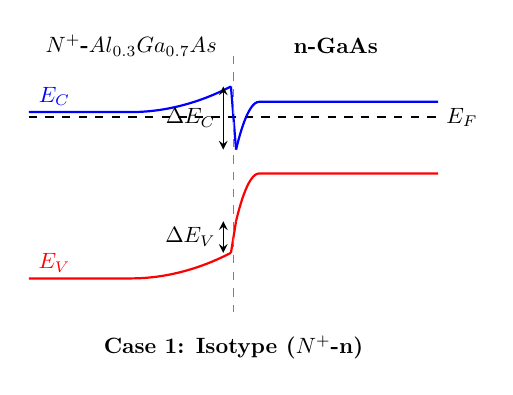
\begin{tikzpicture}[scale=0.65, every node/.style={scale=0.8}]
  % Case 1: N+ - n Isotype
  
  % Fermi level
  \draw[dashed, thick] (-4, 0) -- (4, 0) node[right] {$E_F$};
  
  % Left side (N+ AlGaAs)
  % EC bends up (depletion)
  \draw[thick, blue] (-4, 0.1) -- (-2, 0.1) parabola (-0.05, 0.6);
  % EV bends up
  \draw[thick, red] (-4, -3.15) -- (-2, -3.15) parabola (-0.05, -2.65);
  
  % Right side (n GaAs)
  % EC bends down (accumulation)
  \draw[thick, blue] (4, 0.3) -- (0.5, 0.3) parabola (0.05, -0.633);
  % EV bends down
  \draw[thick, red] (4, -1.1) -- (0.5, -1.1) parabola (0.05, -2.033);
  
  % Interface lines
  \draw[thick, blue] (-0.05, 0.6) -- (0.05, -0.633); % EC spike
  \draw[thick, red] (-0.05, -2.65) -- (0.05, -2.033); % EV step
  \draw[dashed, gray] (0, 1.2) -- (0, -3.8); % Interface vertical line
  
  % Labels
  \node at (-2, 1.4) {\textbf{$\text{N}^+$-$\text{Al}_{0.3}\text{Ga}_{0.7}\text{As}$}};
  \node at (2, 1.4) {\textbf{n-GaAs}};
  \node[blue] at (-3.5, 0.4) {$E_C$};
  \node[red] at (-3.5, -2.85) {$E_V$};
  
  \draw[<->, >=stealth] (-0.2, 0.6) -- (-0.2, -0.633) node[midway, left] {$\Delta E_C$};
  \draw[<->, >=stealth] (-0.2, -2.033) -- (-0.2, -2.65) node[midway, left] {$\Delta E_V$};

  \node at (0, -4.5) {\textbf{Case 1: Isotype ($\text{N}^+$-n)}};
\end{tikzpicture}
\end{minipage}\hfill
\begin{minipage}{0.48\textwidth}
\centering
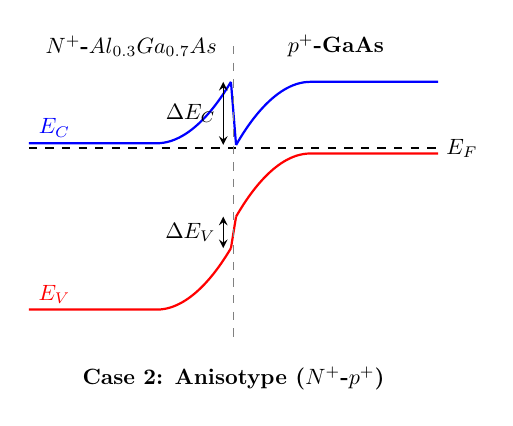
\begin{tikzpicture}[scale=0.65, every node/.style={scale=0.8}]
  % Case 2: N+ - p+ Anisotype
  
  % Fermi level
  \draw[dashed, thick] (-4, 0) -- (4, 0) node[right] {$E_F$};
  
  % Left side (N+ AlGaAs)
  % Depletion region (bends up)
  \draw[thick, blue] (-4, 0.1) -- (-1.5, 0.1) parabola (-0.05, 1.3);
  \draw[thick, red] (-4, -3.15) -- (-1.5, -3.15) parabola (-0.05, -1.95);
  
  % Right side (p+ GaAs)
  % Depletion region (bends down)
  \draw[thick, blue] (4, 1.3) -- (1.5, 1.3) parabola (0.05, 0.067); 
  \draw[thick, red] (4, -0.1) -- (1.5, -0.1) parabola (0.05, -1.333);
  
  % Interface lines
  \draw[thick, blue] (-0.05, 1.3) -- (0.05, 0.067); % EC spike
  \draw[thick, red] (-0.05, -1.95) -- (0.05, -1.333); % EV step
  \draw[dashed, gray] (0, 2) -- (0, -3.8); % Interface vertical line
  
  % Labels
  \node at (-2, 2.0) {\textbf{$\text{N}^+$-$\text{Al}_{0.3}\text{Ga}_{0.7}\text{As}$}};
  \node at (2, 2.0) {\textbf{$\text{p}^+$-GaAs}};
  \node[blue] at (-3.5, 0.4) {$E_C$};
  \node[red] at (-3.5, -2.85) {$E_V$};
  
  \draw[<->, >=stealth] (-0.2, 1.3) -- (-0.2, 0.067) node[midway, left] {$\Delta E_C$};
  \draw[<->, >=stealth] (-0.2, -1.333) -- (-0.2, -1.95) node[midway, left] {$\Delta E_V$};

  \node at (0, -4.5) {\textbf{Case 2: Anisotype ($\text{N}^+$-$\text{p}^+$)}};
\end{tikzpicture}
\end{minipage}
\end{center}

\textbf{Analytical descriptions of the band diagrams:}

\begin{enumerate}
  \item \textbf{Case 1: $\text{N}^+$-$\text{Al}_{0.3}\text{Ga}_{0.7}\text{As}$ on n-GaAs (Isotype):}
  \begin{itemize}
    \item Since both sides are n-type, the Fermi level $E_F$ lies close to the conduction band edges on both sides.
    \item Upon contact, electrons migrate from the wide-bandgap, heavily-doped $\text{N}^+$-AlGaAs into the narrow-bandgap n-GaAs.
    \item This establishes a \textbf{depletion region} (positive space charge, bands bending upward) on the AlGaAs side, and an \textbf{accumulation layer} of electrons (negative space charge, bands bending downward) on the GaAs side.
    \item The conduction band edge displays a sharp spike ($\Delta E_C$) and a notch at the interface.
  \end{itemize}
  \item \textbf{Case 2: $\text{N}^+$-$\text{Al}_{0.3}\text{Ga}_{0.7}\text{As}$ on $\text{p}^+$-GaAs (Anisotype):}
  \begin{itemize}
    \item The Fermi level lies near $E_C$ in AlGaAs and near $E_V$ in GaAs.
    \item Upon alignment, a wide depletion region forms across both materials. Electrons diffuse into the p-side, and holes diffuse into the N-side.
    \item The bands bend strongly in opposite directions (upwards in AlGaAs, downwards in GaAs).
    \item The conduction band exhibits a massive spike of height $\Delta E_C = 1.233$\,eV, acting as a severe barrier to electron transport from N to p. The valence band drops by a step of $\Delta E_V = 0.617$\,eV.
  \end{itemize}
\end{enumerate}


\begin{question}[Question 6]
The lattice spacing of In$_{1-x}$Ga$_x$As$_y$P$_{1-y}$ has been shown to obey Vegard's linear law. This states that for quaternary alloys of the form ABCD where A and B are group III elements (e.g. Al, In and Ga) and C and D are group V elements (e.g. As, P and Sb,) the lattice spacing $a(x,y)$ of the quaternary alloy can be approximated by $a(x,y) = x y \cdot a(BC) + x(1-y) \cdot a(AC) + (1-x)y \cdot a(BD) + (1-x)(1-y) \cdot a(AD)$ Where $a(IJ)$ are the lattice spacing of the binary compounds IJ.\\
(a) Show that for In$_{1-x}$Ga$_x$As$_y$P$_{1-y}$ with $a(\text{GaAs}) = 0.56536$ nm, $a(\text{GaP}) = 0.54512$ nm, $a(\text{InAs}) = 0.60590$ nm and $a(\text{InP}) = 0.58696$ nm, the quaternary lattice spacing becomes $a(x,y) = 0.58696 - 0.04184x + 0.01894y + 0.00130xy$ nm\\
(b) For quaternary alloy that are lattice matched to InP the relation between x and y can be determined by letting $a(x,y) = a(\text{InP})$. Show that since $0 \le x \le 0.47$ the resulting expression can be approximated by $y \approx 2.2x$.\\
(c) A simple empirical relation that gives the band gap energy in terms of x and y is $E_g(x,y) = 1.35 + 0.668x - 1.17y + 0.758x^2 + 0.18y^2 - 0.069xy - 0.322x^2y + 0.03xy^2$ eV. Find the band gap energy and the peak wavelength of In$_{0.74}$Ga$_{0.26}$As$_{0.56}$P$_{0.44}$.
\end{question}

\textbf{\large Solution --- Question 6}

\textbf{(a) Vegard's Law for Quaternary Alloys}

Just as we linearly interpolate between two materials for a ternary alloy, we use a 2D interpolation for a four-element (quaternary) alloy. The lattice constant of $\text{In}_{1-x}\text{Ga}_x\text{As}_y\text{P}_{1-y}$ is a weighted average of the four possible binary crystal combinations (GaAs, GaP, InAs, and InP). The weighting corresponds to the probability of finding those specific pairs in the crystal lattice.

Applying Vegard's law to the generalized quaternary model:
\begin{equation*}
  a(x,y) = x y \cdot a(\text{GaAs}) + x(1-y) \cdot a(\text{GaP}) + (1-x)y \cdot a(\text{InAs}) + (1-x)(1-y) \cdot a(\text{InP})
\end{equation*}
Rather than substituting the numerical values immediately, it is algebraically cleaner to expand the expression symbolically first:
\begin{align*}
  a(x,y) &= xy \cdot a_{\text{GaAs}} + x(1-y) \cdot a_{\text{GaP}} + (1-x)y \cdot a_{\text{InAs}} + (1-x)(1-y) \cdot a_{\text{InP}} \\
  &= xy \cdot a_{\text{GaAs}} + x \cdot a_{\text{GaP}} - xy \cdot a_{\text{GaP}} + y \cdot a_{\text{InAs}} - xy \cdot a_{\text{InAs}} + a_{\text{InP}} - x \cdot a_{\text{InP}} - y \cdot a_{\text{InP}} + xy \cdot a_{\text{InP}}
\end{align*}
Now, we group the terms by the linear coefficients ($x, y$) and the non-linear cross-term ($xy$):
\begin{align*}
  a(x,y) &= a_{\text{InP}} + x(a_{\text{GaP}} - a_{\text{InP}}) + y(a_{\text{InAs}} - a_{\text{InP}}) + xy(a_{\text{GaAs}} - a_{\text{GaP}} - a_{\text{InAs}} + a_{\text{InP}})
\end{align*}
With the analytical form simplified, we now substitute the measured binary lattice constants (in nm):
\begin{itemize}
    \item $a_{\text{InP}} = 0.58696$
    \item $a_{\text{GaP}} - a_{\text{InP}} = 0.54512 - 0.58696 = -0.04184$
    \item $a_{\text{InAs}} - a_{\text{InP}} = 0.60590 - 0.58696 = 0.01894$
    \item $a_{\text{GaAs}} - a_{\text{GaP}} - a_{\text{InAs}} + a_{\text{InP}} = 0.56536 - 0.54512 - 0.60590 + 0.58696 = 0.00130$
\end{itemize}
Yielding the final equation:
\begin{equation*}
  a(x,y) = 0.58696 - 0.04184 x + 0.01894 y + 0.00130 x y\,\text{nm}
\end{equation*}

\textbf{(b) The Physics of Lattice Matching to an InP Substrate}

When fabricating semiconductor lasers, the active quaternary layer must be grown on a thick, stable structural foundation (the substrate). Here, InP is the substrate. To prevent structural defects and non-radiative recombination at the interface, the active layer's lattice constant $a(x,y)$ must perfectly match the InP substrate $a_{\text{InP}} = 0.58696\,\text{nm}$. 

Setting $a(x,y) = 0.58696$:
\begin{equation*}
  0.58696 - 0.04184 x + 0.01894 y + 0.00130 x y = 0.58696
\end{equation*}
\begin{equation*}
  -0.04184 x + 0.01894 y + 0.00130 x y = 0
\end{equation*}
This equation links the two compositional degrees of freedom ($x$ and $y$). Because the non-linear "bowing" coefficient ($0.00130$) is two orders of magnitude smaller than the linear terms, the $xy$ term is physically negligible:
\begin{equation*}
  0.01894 y \approx 0.04184 x \quad\Longrightarrow\quad y \approx \frac{0.04184}{0.01894} x \approx \boxed{2.2 x}
\end{equation*}

\textbf{(c) Band gap and peak emission wavelength}

We are given a specific alloy: $\text{In}_{0.74}\text{Ga}_{0.26}\text{As}_{0.56}\text{P}_{0.44}$.
Matching this to the general form $\text{In}_{1-x}\text{Ga}_x\text{As}_y\text{P}_{1-y}$, we find the compositional fractions:
\begin{equation*}
  1-x = 0.74 \implies x = 0.26 \quad \text{and} \quad y = 0.56
\end{equation*}
\textit{Notice that $y \approx 2.2x$ ($0.56 \approx 2.2 \times 0.26 = 0.572$), meaning this specific alloy was explicitly engineered to be lattice-matched to InP!}

Evaluating the empirical bandgap formula with $x=0.26$ and $y=0.56$:
\begin{align*}
  E_g(0.26, 0.56) &= 1.35 + 0.668(0.26) - 1.17(0.56) + 0.758(0.26)^2 + 0.18(0.56)^2 \\
  &\quad - 0.069(0.26)(0.56) - 0.322(0.26)^2(0.56) + 0.03(0.26)(0.56)^2
\end{align*}
\begin{equation*}
  E_g \approx \boxed{0.956\,\text{eV}}
\end{equation*}

The corresponding peak emission wavelength is:
\begin{equation*}
  \lambda_p = \frac{hc}{E_g} = \frac{1.24\,\text{eV}\cdot\mu\text{m}}{0.956\,\text{eV}} \approx \boxed{1.30\,\mu\text{m}}
\end{equation*}

\begin{question}[Question 7]
\noindent\begin{minipage}[c]{0.60\linewidth}
The active layer of a semiconductor laser is made of In$_{1-x}$Ga$_x$As$_y$P$_{1-y}$ while the upper and lower cladding layers are made of InP (as shown at the inset of the figure).\\[1ex]
(a) If the energy gap $E_g = 1.3 - 0.72 y + 0.12 y^2$ (eV), then find $y$ and $x$ to emit light at 1.3 \si{\micro\meter}.\\
(b) Use the figure shown (which plots the refractive index of the active layer versus photon energy at different $y$ in steps of 0.1) to find the thickness of the active layer that maximizes optical confinement under single-mode condition.
\end{minipage}\hfill
\begin{minipage}[c]{0.36\linewidth}
  \centering
  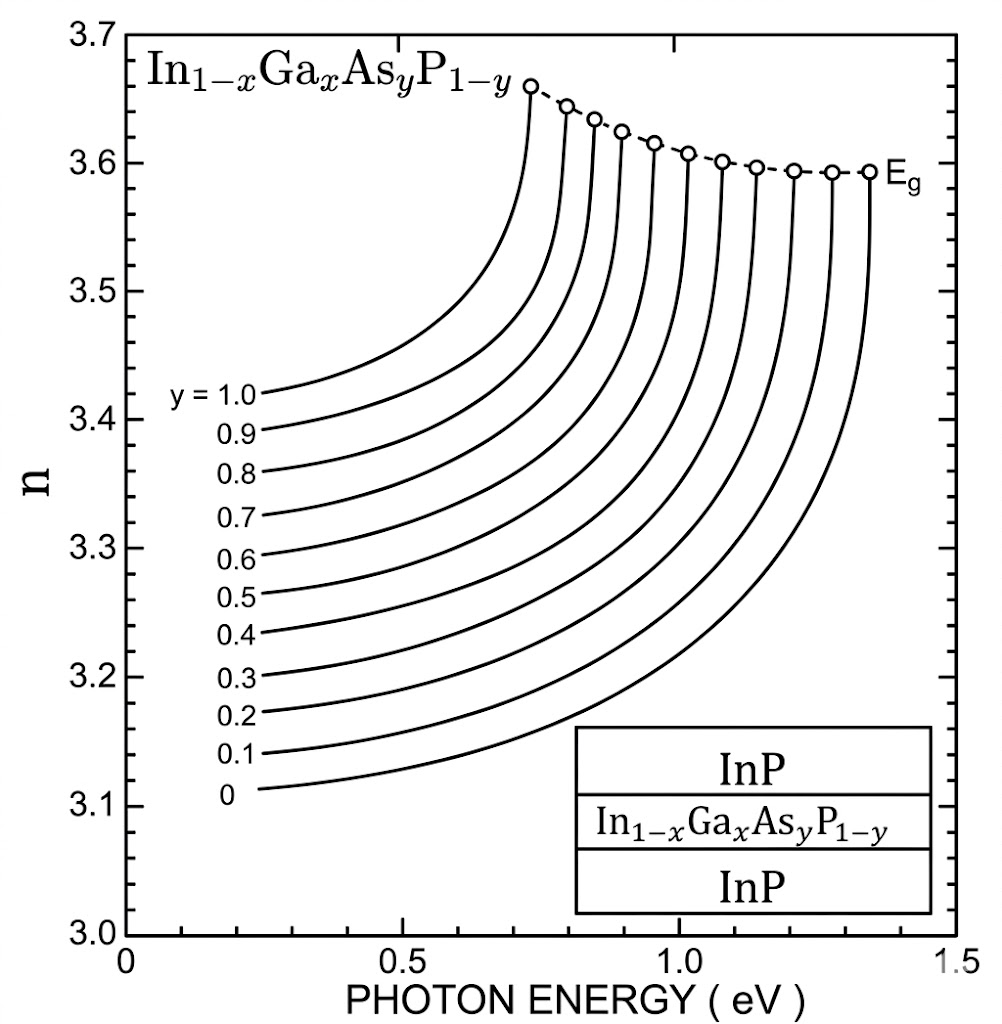
\includegraphics[width=\linewidth]{../Figures/Sheet 7/q7.jpg}
\end{minipage}
\end{question}

\textbf{\large Solution --- Question 7}

\textbf{(a) Engineering the Active Layer Composition ($x$ and $y$)}

To design a laser emitting at a specific telecommunications wavelength ($\lambda_L = 1.3\,\mu\text{m}$), we first determine the required bandgap energy of the active layer. Using the photon energy relation:
\begin{equation*}
  E_g = \frac{hc}{\lambda_L} = \frac{1.24\,\text{eV}\cdot\mu\text{m}}{1.3\,\mu\text{m}} \approx 0.954\,\text{eV} \approx 0.95\,\text{eV}
\end{equation*}

We are given the empirical relation for the bandgap of the quaternary alloy $\text{In}_{1-x}\text{Ga}_x\text{As}_y\text{P}_{1-y}$ as a function of the Arsenic fraction ($y$):
\begin{equation*}
  1.3 - 0.72y + 0.12y^2 = 0.95 \quad\Longrightarrow\quad 0.12y^2 - 0.72y + 0.35 = 0
\end{equation*}
Solving this quadratic equation for $y$:
\begin{equation*}
  y = \frac{0.72 \pm \sqrt{(-0.72)^2 - 4(0.12)(0.35)}}{2(0.12)} = \frac{0.72 \pm \sqrt{0.5184 - 0.168}}{0.24} = \frac{0.72 \pm \sqrt{0.3504}}{0.24}
\end{equation*}
Taking the physically meaningful root (since $0 \le y \le 1$):
\begin{equation*}
  y = \frac{0.72 - 0.592}{0.24} \approx 0.533 \approx 0.53
\end{equation*}

To ensure the active layer does not crack or form non-radiative defects, it must be lattice-matched to the thick InP substrate. From our previous derivation (Question 6), the lattice matching condition for InP is $y \approx 2.2x$. We use this constraint to find the required Gallium fraction ($x$):
\begin{equation*}
  x \approx \frac{y}{2.2} = \frac{0.533}{2.2} \approx 0.242 \approx 0.24
\end{equation*}
Thus, the perfectly lattice-matched active layer composition that emits at $1.3\,\mu\text{m}$ is $\text{In}_{0.76}\text{Ga}_{0.24}\text{As}_{0.53}\text{P}_{0.47}$.

\textbf{(b) Waveguide thickness for maximum optical confinement}

In a semiconductor laser, the active layer also serves as a dielectric waveguide. A thicker active layer increases the optical confinement factor ($\Gamma$), pulling more of the optical mode into the gain region and increasing efficiency. However, if the layer is too thick, it will begin to support higher-order transverse modes (like TE$_1$), ruining the laser's beam quality. 

To maximize confinement while guaranteeing strict single-mode operation, we set the waveguide thickness exactly at the cutoff condition for the first higher-order mode. For a symmetric slab waveguide, this occurs when the normalized frequency $V = \pi$.

First, we determine the refractive indices from the provided plot at $E_g = 0.95\,\text{eV}$:
\begin{itemize}
    \item \textbf{Active Core ($y=0.53$):} Interpolating between the $y=0.5$ and $y=0.6$ curves gives $n_{\text{active}} \approx 3.6$.
    \item \textbf{Cladding (InP, $y=0$):} Following the $y=0$ curve gives $n_{\text{cladding}} \approx 3.2$.
\end{itemize}

Setting $V = \pi$:
\begin{equation*}
  V = \frac{2\pi}{\lambda_L} d \sqrt{n_{\text{active}}^2 - n_{\text{cladding}}^2} = \pi \quad\Longrightarrow\quad d = \frac{\lambda_L}{2\sqrt{n_{\text{active}}^2 - n_{\text{cladding}}^2}}
\end{equation*}
Substituting our values:
\begin{equation*}
  d = \frac{1.3\,\mu\text{m}}{2\sqrt{3.6^2 - 3.2^2}} = \frac{1.3}{2\sqrt{12.96 - 10.24}} = \frac{1.3}{2\sqrt{2.72}} = \frac{1.3}{2(1.649)} \approx \boxed{0.39\,\mu\text{m}}
\end{equation*}
By engineering the active layer thickness to exactly $0.39\,\mu\text{m}$, we achieve the maximum possible optical overlap with the gain medium without sacrificing single-mode beam quality.

